% !TeX root = it-governance-risk-compliance.tex
% !TeX encoding = UTF-8
\chapter{KPI, KRI, dan Pelaporan ke Direksi}

\section*{Tujuan Pembelajaran}
\begin{itemize}
  \item Membedakan KPI, KRI, dan KCI, lalu memilih indikator yang memicu tindakan.
  \item Menetapkan ambang batas KRI yang selaras dengan \textit{risk appetite}.
  \item Menyusun laporan GRC satu halaman yang dapat dipakai direksi untuk mengambil keputusan.
\end{itemize}

\section{Pendahuluan}

Misalkan direksi Medikara menerima laporan bulanan Teknologi Informasi (TI) setebal 40 halaman.
Bila satu halaman dibaca 2 menit, satu pembaca memerlukan 80 menit. Laporan itu mencatat banyak
kegiatan, tetapi tidak menjawab dua pertanyaan direksi: apakah risiko akses vendor membaik, dan
keputusan apa yang diminta? Panjang laporan tidak menggantikan hubungan antara ukuran, tujuan,
dan tindakan.

Bab 5 sudah menetapkan batas risiko Medikara. Bab 8 sampai Bab 12 sudah merancang target,
kontrol, dan cara mengujinya. Bab ini mengubah semuanya menjadi sinyal yang dibaca secara berkala.
Key Performance Indicator (KPI) mengukur pencapaian hasil. Key Risk Indicator (KRI) memberi sinyal
perubahan paparan risiko. Key Control Indicator (KCI) mengukur pelaksanaan kontrol. Hasil kerja
bab ini adalah katalog indikator, \textit{dashboard}, dan laporan Governance, Risk, and Compliance
(GRC) satu halaman untuk tonggak C4 capstone.

Bab ini memakai panduan pengukuran NIST SP 800-55 Volume 1 dari National Institute of Standards
and Technology (NIST), makalah Committee of Sponsoring Organizations of the Treadway Commission
(COSO) tentang KRI, dan Cybersecurity Framework (CSF) 2.0. Objektif Control Objectives for
Information and Related Technologies (COBIT) 2019 hanya disinggung secara umum, karena naskah
rincinya tidak dibaca langsung oleh bab ini. Ambang dan angka Medikara merupakan keputusan
skenario, bukan angka wajib standar \cite{c13-nist80055v1,c13-coso-kri,nistcsf2,c04-gmo}.

Gambar~\ref{fig:ch13-alur} menunjukkan urutan kerja bab ini.

\begin{figure}[!htb]
  \centering
  \begin{tikzpicture}[node distance=5mm, kotak/.style={draw, rounded corners, align=center, text width=2.3cm, minimum height=1.55cm, font=\scriptsize, execute at begin node={\hyphenpenalty=10000}}, panah/.style={-{Stealth[length=2mm]}, thick}]
  \node[kotak,fill=praditagreen!15] (t0) {\textbf{Tujuan dan risiko}\\[1pt]{\tiny\mdseries R-01 sampai \mbox{R-12},\\ batas Bab 5}};
  \node[kotak,fill=blue!8] (t1) [right=of t0] {\textbf{Definisi dan data}\\[1pt]{\tiny\mdseries pembilang, penyebut, sumber}};
  \node[kotak,fill=orange!12] (t2) [right=of t1] {\textbf{Ambang dan tindakan}\\[1pt]{\tiny\mdseries hijau, kuning, merah, pemilik}};
  \node[kotak,fill=green!10] (t3) [right=of t2] {\textbf{Keputusan dan tinjauan}\\[1pt]{\tiny\mdseries opsi, biaya, tenggat}};
  \draw[panah] (t0) -- (t1);
  \draw[panah] (t1) -- (t2);
  \draw[panah] (t2) -- (t3);
  \draw[panah] (t3.south) -- ++(0,-0.45) -| (t0.south) node[pos=0.25, below, font=\scriptsize] {hasil keputusan mengubah risiko dan indikator pada periode berikutnya};
\end{tikzpicture}

  \caption{Alur dari tujuan dan risiko sampai keputusan}
  \label{fig:ch13-alur}
\end{figure}

\IfFileExists{../figures/ch13-diagram-konsep.png}{%

Gambar \ref{fig:ch13-ilustrasi-bab} merangkum hubungan komponen dan konsep utama bab ini.
\begin{figure}[!htb]
  \centering
  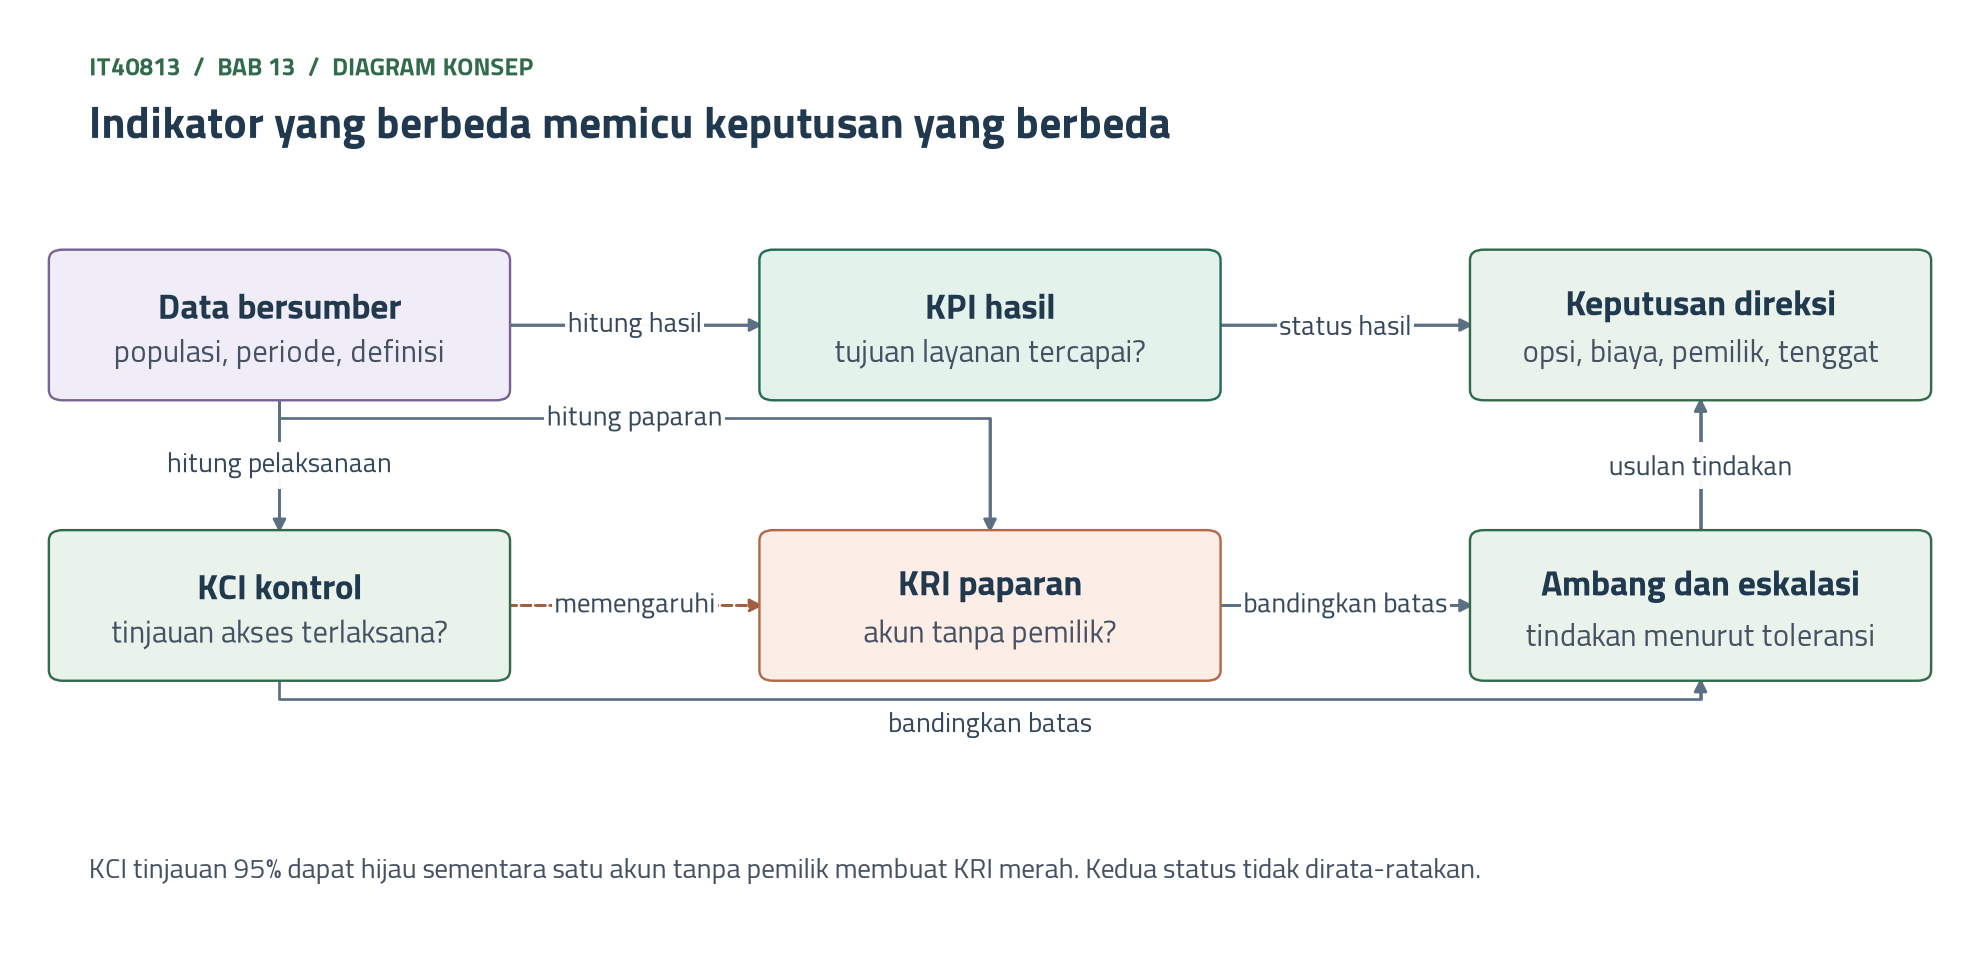
\includegraphics[width=\textwidth]{../figures/ch13-diagram-konsep.png}
  \caption{Indikator yang berbeda memicu keputusan yang berbeda}
  \label{fig:ch13-ilustrasi-bab}
\end{figure}
}{}

\section{KPI, KRI, dan KCI}

\subsection*{Tiga pertanyaan yang berbeda}

KPI menjawab apakah tujuan tercapai. KRI menjawab apakah paparan mendekati atau melewati batas.
KCI menjawab apakah kontrol dijalankan. COSO mengingatkan bahwa laporan kinerja sering berfokus
pada hasil yang sudah terjadi, sehingga belum tentu memberi peringatan dini. KRI dipakai untuk
memberi sinyal awal ketika paparan risiko meningkat \cite{c13-coso-kri}. Bab 5 mencatat fungsi
yang sama: ukuran seperti KRI menunjukkan bagian yang melewati toleransi atau yang masih berada
di dalamnya \cite{c05-nist-ir8286r1}.

Analogi kendaraan pengantar obat menunjukkan perbedaannya. Waktu tiba di apotek menunjukkan
hasil. Suhu mesin menunjukkan potensi gangguan. Buku servis rutin menunjukkan pelaksanaan kontrol.
Ketiganya membantu keputusan berbeda, dan tidak satu pun menggantikan yang lain.

Dua contoh pada Medikara:
\begin{enumerate}
  \item Misalkan 12 acara pelatihan keamanan hanya menjangkau 30 dari 100 pegawai prioritas, atau
  30 persen. Jumlah acara mengukur kegiatan. Cakupannya menunjukkan 70 pegawai belum terjangkau,
  dan itu pun belum membuktikan perilaku berubah.
  \item Misalkan 114 dari 120 akun vendor ditinjau tepat waktu pada Oktober 2026. KCI-nya 95 persen
  dan berstatus hijau. Pada bulan yang sama, 1 akun aktif belum memiliki pemilik. KRI-nya merah
  menurut batas nol pada Bab 5.
\end{enumerate}

Tabel~\ref{tab:ch13-jenis-indikator} merangkum ketiga jenis indikator beserta keputusan yang
dipicu.

\begin{table}[!htb]
  \centering\small
  \caption{Jenis indikator Medikara, Oktober 2026 (misalkan)}\label{tab:ch13-jenis-indikator}
  \begin{tabularx}{\textwidth}{|>{\raggedright\arraybackslash}p{0.08\textwidth}|>{\raggedright\arraybackslash}p{0.22\textwidth}|>{\raggedright\arraybackslash}X|>{\raggedright\arraybackslash}X|}
    \hline
    \textbf{Jenis} & \textbf{Pertanyaan} & \textbf{Ukuran contoh} & \textbf{Keputusan yang dipicu}
    \\ \hline
    KPI & Apakah hasil tercapai? & Waktu tunggu pendaftaran 28 menit, target 25 menit & Alur dan
    jadwal petugas diubah atau dipertahankan? \\ \hline
    KRI & Apakah paparan mendekati batas? & 1 akun vendor tanpa pemilik, batas 0 akun & Akun
    dibekukan atau diberi pengecualian darurat? \\ \hline
    KCI & Apakah kontrol dijalankan? & 114 dari 120 akun ditinjau tepat waktu & Daftar akun
    diperbaiki atau peninjau ditambah? \\ \hline
  \end{tabularx}
\end{table}

Dua hal pada indikator sering tertukar: KRI dan KCI. Pembagiannya begini. KCI mengukur pekerjaan
organisasi. KRI mengukur keadaan yang dihadapi organisasi. Cakupan peninjauan dapat mencapai 100
persen, sementara peninjau tetap menemukan akun tanpa pemilik. Klasifikasi mengikuti pertanyaan,
bukan nama datanya. Jumlah menit gangguan menjadi KRI bila dibandingkan dengan batas 2 jam per
bulan pada Bab 5. Data yang sama menjadi KPI bila kepala operasi TI memakainya untuk menilai
target waktu pulih.

Diagram konsep pada awal bab merangkum alurnya. Data bersumber memuat populasi, periode, dan
definisi. Dari data itu lahir KPI hasil, KCI kontrol, dan KRI paparan. Nilai dibandingkan dengan
batas pada ambang dan eskalasi, yaitu tindakan menurut toleransi. Status hasil dan usulan tindakan
lalu masuk ke keputusan direksi, yang memuat opsi, biaya, pemilik, dan tenggat.

Pertanyaan kemudian muncul: mengapa diagram itu memuat panah dari KCI ke KRI? Bab 5 memberi
angkanya. Pengandaian kasarnya: penurunan peluang R-01 sebanding dengan cakupan AC-01, dari 0,2
menuju 0,05. Hasilnya sebagai berikut:
\begin{enumerate}
  \item Cakupan 85 persen menghasilkan peluang $0{,}2 - 0{,}15 \times 0{,}85 = 0{,}0725$, dengan
  harapan kerugian Rp36,25 juta dari kerugian rata-rata Rp500 juta.
  \item Cakupan 90 persen menghasilkan peluang 0,065 dan harapan kerugian Rp32,5 juta, sama dengan
  Bab 5. Cakupan 95 persen menghasilkan 0,0575 dan Rp28,75 juta. Sasaran Rp25 juta baru tercapai
  pada cakupan penuh.
\end{enumerate}

Hubungan itu pengandaian, bukan hukum sebab akibat. Selisih 5 persen cakupan terakhir, yaitu 6
akun, bernilai Rp3,75 juta per tahun. Angka kecil itu tidak meniadakan kewajiban nol akun tanpa
pemilik, karena batas Bab 5 tidak ditetapkan dari harapan kerugian saja.

\begin{kasus}[title={Kasus Medikara Health: Indikator Hijau, Risiko Merah}]
Misalkan kepala operasi TI melaporkan cakupan AC-01 naik dari 85 persen menjadi 95 persen dalam
tiga bulan. Angka itu benar. Pemilik Medikara+ lalu membaca KRI pada halaman yang sama: 1 akun
vendor aktif belum memiliki pemilik. Angka ini juga benar, dan statusnya merah.

Keputusan membaca dua status secara terpisah punya dua konsekuensi. Pertama, perbaikan cakupan
tetap terlihat, sehingga kerja tim operasi tidak hilang dari laporan. Kedua, akun itu tetap
divalidasi dalam 1 hari kerja lalu dibekukan, walaupun hanya 1 dari 120 akun, atau sekitar 0,8
persen. Warna hijau pada satu baris tidak membayar warna merah pada baris lain.
\end{kasus}

\subsection*{Indikator yang mendahului dan yang tertinggal}

Indikator yang mendahului memberi peringatan sebelum kejadian. Indikator yang tertinggal
menggambarkan hasil sesudah kejadian. COSO menyarankan penelusuran mundur: dari kejadian risiko ke
kejadian antara, lalu ke akar penyebab. Data pada titik yang lebih awal berpotensi menjadi KRI yang
mendahului \cite{c13-coso-kri}. Makin dini sinyalnya, makin panjang waktu untuk bertindak.

Analogi prakiraan banjir membantu. Tinggi air di bendungan hulu memberi waktu mengungsi. Jumlah
rumah terendam hanya menghitung akibat. Keduanya berguna, tetapi hanya yang pertama dapat mencegah
kerugian pada hari itu.

Gambar~\ref{fig:ch13-rantai} menerapkan penelusuran itu pada R-01. Kode IK-01 sampai IK-12 adalah
indikator bab ini, yang dirinci pada seksi metrik.

\begin{figure}[!htb]
  \centering
  \begin{tikzpicture}[node distance=4.5mm, tahap/.style={draw, rounded corners, align=center, text width=2.4cm, minimum height=1.5cm, font=\scriptsize}, ukur/.style={draw, align=center, text width=2.4cm, minimum height=1.25cm, font=\scriptsize, fill=blue!8}, panah/.style={-{Stealth[length=2mm]}, thick}]
  \node[tahap,fill=blue!8] (a) {\textbf{Akar penyebab}\\[1pt]{\tiny\mdseries tanggal berakhir tidak masuk daftar}};
  \node[tahap,fill=orange!12] (b) [right=of a] {\textbf{Kejadian antara}\\[1pt]{\tiny\mdseries akun aktif melewati masa berlaku}};
  \node[tahap,fill=red!22] (c) [right=of b] {\textbf{Kejadian risiko}\\[1pt]{\tiny\mdseries akun membaca data pasien tanpa tugas}};
  \node[tahap,fill=gray!35] (d) [right=of c] {\textbf{Akibat}\\[1pt]{\tiny\mdseries pemberitahuan dan kerugian}};
  \draw[panah] (a) -- (b);
  \draw[panah] (b) -- (c);
  \draw[panah] (c) -- (d);
  \node[ukur] (ua) [below=6mm of a] {\textbf{KCI IK-07}\\{\tiny\mdseries cakupan peninjauan AC-01}};
  \node[ukur] (ub) [below=6mm of b] {\textbf{KRI IK-01, IK-02}\\{\tiny\mdseries akun tanpa pemilik; lewat masa berlaku}};
  \node[ukur] (uc) [below=6mm of c] {\textbf{Tinjauan \textit{log}}\\{\tiny\mdseries 247 dari 260 tinjauan mingguan (Bab 8)}};
  \node[ukur] (ud) [below=6mm of d] {\textbf{KPI IK-11}\\{\tiny\mdseries pemberitahuan tepat waktu}};
  \draw[-, dashed] (a) -- (ua);
  \draw[-, dashed] (b) -- (ub);
  \draw[-, dashed] (c) -- (uc);
  \draw[-, dashed] (d) -- (ud);
  \draw[panah] ([yshift=-5mm]ua.south west) -- node[below, font=\scriptsize] {sinyal makin terlambat, waktu untuk bertindak makin pendek} ([yshift=-5mm]ud.south east);
\end{tikzpicture}

  \caption{Rantai kejadian R-01 dan indikator pada tiap titik (misalkan)}
  \label{fig:ch13-rantai}
\end{figure}

Dua contoh membedakan keduanya:
\begin{enumerate}
  \item Bab 5 memberi contoh akun melewati masa berlaku naik dari 1 menjadi 5 dalam sebulan.
  Kenaikan itu memicu pemeriksaan sebelum insiden terulang. Indikator ini mendahului kejadian.
  \item Ketepatan pemberitahuan hanya memiliki nilai bila ada insiden wajib. Misalkan Agustus
  memuat 1 pemberitahuan yang tepat waktu, dan dua bulan berikutnya tidak ada. Indikator ini
  tertinggal. Ia tidak memberi peringatan, tetapi tetap perlu karena K-04 merupakan kewajiban.
\end{enumerate}

Hubungan waktu tidak otomatis membuktikan sebab akibat. Misalkan akun lewat masa berlaku turun 2,
1, 0 dan akun tanpa pemilik turun 3, 2, 1. Tiga titik data belum membuktikan yang satu menyebabkan
yang lain. COSO juga mengingatkan bahwa KRI tidak mengelola risiko, dan rancangan yang buruk dapat
memberi rasa aman palsu. Kemampuan prediksi tiap KRI karena itu dinilai terus-menerus
\cite{c13-coso-kri}.

\subsection*{Balanced Scorecard dan keseimbangan ukuran}

Kaplan dan Norton memperkenalkan Balanced Scorecard pada 1992. Alasannya, ukuran keuangan
tradisional dapat memberi sinyal yang menyesatkan bagi perbaikan berkelanjutan dan inovasi
\cite{c13-kaplan1992}. Rumusan umumnya menyandingkan empat perspektif: keuangan, pelanggan, proses
internal, serta inovasi dan pembelajaran. Teks utuh artikel tidak terbuka, sehingga daftar ini
tidak dikutip dari artikel. Bab ini tidak memakainya sebagai sistem
manajemen, melainkan sebagai pemeriksaan keseimbangan. Portofolio yang hanya berisi kontrol
keamanan tidak menjawab apakah pasien terlayani.

Analogi rapor sekolah menjelaskan gunanya. Nilai ujian, kehadiran, dan catatan perilaku dibaca
bersama. Nilai ujian tinggi dengan kehadiran 50 persen memberi pesan yang berbeda dari nilai yang
sama dengan kehadiran penuh.

Dua contoh ketidakseimbangan:
\begin{enumerate}
  \item Bab 2 mengandaikan investasi Rp8 miliar dengan kemajuan pekerjaan 90 persen, tetapi waktu
  tunggu hanya berubah dari 40 ke 38 menit. Capaian manfaatnya 2 dari 15 menit, atau 13,3 persen.
  Laporan proyek saja akan terlihat hijau.
  \item Misalkan waktu tunggu Oktober 28 menit. Capaian manfaatnya naik menjadi $12 \div 15 = 80$
  persen. Pada bulan yang sama, baru 1 dari 2 uji rumah sakit lulus. Layanan membaik, tetapi
  kesiapan pulihnya belum.
\end{enumerate}

Tabel~\ref{tab:ch13-keseimbangan} memeriksa keseimbangan portofolio Medikara. Kata ``pasien''
menggantikan ``pelanggan'' karena sesuai dengan konteks layanan.

\begin{table}[!htb]
  \centering\small
  \caption{Pemeriksaan keseimbangan portofolio Medikara, Oktober 2026 (misalkan)}
  \label{tab:ch13-keseimbangan}
  \begin{tabularx}{\textwidth}{|>{\raggedright\arraybackslash}p{0.19\textwidth}|>{\raggedright\arraybackslash}X|>{\raggedright\arraybackslash}p{0.13\textwidth}|>{\raggedright\arraybackslash}p{0.27\textwidth}|}
    \hline
    \textbf{Perspektif} & \textbf{Pertanyaan} & \textbf{Indikator} & \textbf{Nilai} \\ \hline
    Keuangan & Apakah peluang kerugian besar berada di dalam batas? & IK-04 & 1 skenario di atas
    batas 2 persen \\ \hline
    Pasien & Apakah layanan lebih cepat dan tersedia? & IK-03, IK-12 & 100 menit gangguan; tunggu
    28 menit \\ \hline
    Proses internal & Apakah kontrol berjalan dan bekerja? & IK-07, IK-08 & Cakupan 95 persen; 10
    dari 12 uji lulus \\ \hline
    Pembelajaran & Apakah temuan menghasilkan perbaikan yang teruji? & IK-10 & 9 dari 10 temuan
    tertutup \\ \hline
  \end{tabularx}
\end{table}

\section{Merancang Indikator yang Baik}

\subsection*{Kartu definisi}

NIST membedakan penilaian dari pengukuran. Penilaian mengevaluasi atau menimbang terhadap kriteria.
Pengukuran menghasilkan nilai kuantitatif. Metrik memakai hasil pengukuran untuk melacak kemajuan,
membantu keputusan, dan memperbaiki kinerja terhadap sasaran. Metrik yang bermakna bersifat
objektif, akurat, presisi, terikat pada titik waktu, dapat diulang, dan sebanding dengan pengukuran
sebelumnya. Dokumentasinya mencatat pihak yang bertanggung jawab, sumber data, dan bentuk laporan
\cite{c13-nist80055v1}. Volume 2 melanjutkannya menjadi program pengukuran \cite{c13-nist80055v2}.

Analogi nilai kelas menunjukkan bahaya penyebut yang kabur. Nilai rata-rata 90 berbeda maknanya
bila hanya menghitung siswa yang hadir, bukan seluruh peserta. Perubahan cara menghitung dapat
memperbaiki angka tanpa mengubah kemampuan kelas.

Dua contoh tentang penyebut:
\begin{enumerate}
  \item Bab 12 mencatat laporan unit TI berbunyi 108 dari 108 akun. Penyebut yang benar adalah 120
  akun pada daftar penugasan, sehingga cakupannya $108 / 120 = 90$ persen. Selisih 12 akun tidak
  pernah ditinjau. Kedua angka benar, tetapi hanya satu yang menjawab pertanyaan direksi.
  \item Misalkan sesudah perbaikan, pembilang diperketat menjadi akun yang ditinjau tepat waktu
  dalam bulan itu. Agustus menghasilkan $102 / 120 = 85$ persen, lebih rendah daripada 90 persen.
  Angka turun karena definisi menjadi lebih ketat, bukan karena kontrol memburuk. Perubahan definisi
  itu dicatat, dan tren lama tidak disambung tanpa catatan.
\end{enumerate}

Tabel~\ref{tab:ch13-definisi} memperlihatkan kartu definisi lengkap untuk satu indikator. Katalog
contoh seluruh indikator ada di \berkas{sources/chapter13/katalog-indikator.csv}.

\begin{table}[!htb]
  \centering\small
  \caption{Kartu definisi IK-07 Cakupan peninjauan AC-01 (misalkan)}\label{tab:ch13-definisi}
  \begin{tabularx}{\textwidth}{|>{\raggedright\arraybackslash}p{0.24\textwidth}|>{\raggedright\arraybackslash}X|}
    \hline
    \textbf{Unsur} & \textbf{Isi} \\ \hline
    Pertanyaan & Apakah peninjauan akses vendor dijalankan tepat waktu pada seluruh akun? \\ \hline
    Pembilang & Akun aktif yang ditinjau dalam bulan berjalan, dengan tanggal bukti \\ \hline
    Penyebut & Semua akun aktif pada daftar penugasan: 120 akun pada 5 rumah sakit \\ \hline
    Sumber & Daftar penugasan dan catatan peninjauan, bukan daftar dari sistem yang diperiksa \\
    \hline
    Frekuensi dan tanggal data & Bulanan; ekstrak pada hari kerja terakhir, versi disimpan \\ \hline
    Pemilik informasi & Kepala operasi TI sebagai pemilik tindakan \\ \hline
    Pengumpul dan penerima & Staf TI mengumpulkan; pemilik Medikara+ sebagai pemilik R-01 menerima
    \\ \hline
    Ambang & Minimal 95 persen hijau; 90 sampai kurang dari 95 kuning; kurang dari 90 merah \\
    \hline
    Tindakan & Periksa kelengkapan daftar akun; koreksi kuning dalam 5 hari kerja; merah dieskalasi
    \\ \hline
    Pemeriksa mutu & Audit internal mencocokkan sampel 30 akun (Bab 12) \\ \hline
  \end{tabularx}
\end{table}

\subsection*{Nol, kosong, dan tidak berlaku}

Tiga keadaan pada data sering tertukar. Pembagiannya begini. Nol yang sah berarti data lengkap dan
hasilnya nol. Tidak berlaku berarti penyebutnya nol karena kewajiban tidak muncul. Data tidak
tersedia berarti data kosong atau ekstrak tidak lengkap. Tabel~\ref{tab:ch13-keadaan} memberi
contohnya.

\begin{table}[!htb]
  \centering\small
  \caption{Tiga keadaan data pada \textit{dashboard} (misalkan)}\label{tab:ch13-keadaan}
  \begin{tabularx}{\textwidth}{|>{\raggedright\arraybackslash}p{0.2\textwidth}|>{\raggedright\arraybackslash}X|>{\raggedright\arraybackslash}p{0.3\textwidth}|}
    \hline
    \textbf{Keadaan} & \textbf{Contoh} & \textbf{Status} \\ \hline
    Nol yang sah & 0 baris kewajiban lewat tenggat pada Oktober, register lengkap & Dinilai menurut
    ambang: hijau \\ \hline
    Tidak berlaku & 0 pemberitahuan wajib pada September, sehingga penyebut nol & Tidak berlaku;
    bukan 100 persen \\ \hline
    Data tidak tersedia & Ekstrak akun Bogor gagal, sehingga 20 dari 120 akun tidak terbaca & Belum
    dapat dinilai; bukan hijau \\ \hline
  \end{tabularx}
\end{table}

Pembagian ini punya dua konsekuensi yang dapat dihitung. Pertama, ketepatan pemberitahuan tiga
bulan adalah 1 dari 1, bukan 3 dari 3. Menuliskan 100 persen untuk tiap bulan membuat dua bulan
tanpa kejadian terlihat seperti dua bukti keberhasilan. Kedua, bila ekstrak Bogor gagal, laporan
``nol akun tanpa pemilik'' hanya mencakup 100 dari 120 akun, atau 83,3 persen. Sebaran 120 akun
mengikuti Bab 12. Nol itu tidak dapat dibaca hijau.

\subsection*{Empat jenis ukuran menurut NIST}

NIST memakai pembagian lain: ukuran implementasi, efektivitas, efisiensi, dan dampak
\cite{c13-nist80055v1}. Ukuran implementasi memperlihatkan kemajuan kontrol, biasanya dalam
persentase, misalnya Multi-Factor Authentication (MFA) pada 108 dari 120 akun. Kontrol yang ada
belum tentu bekerja. Ukuran efektivitas menilai seberapa baik kontrol bekerja, misalnya 29 dari 36
uji pemulihan lulus. Ukuran efisiensi melihat ketepatan waktu kontrol, misalnya akun dicabut paling
lambat 1 hari kerja. Ukuran dampak menyatakan akibat bagi misi, misalnya harapan kerugian R-01
Rp28,75 juta, yang masih bergantung pada pengandaian Bab 5.

Dua pembagian itu menjawab hal berbeda. KPI, KRI, dan KCI menjelaskan pertanyaan yang dijawab. Jenis
NIST menjelaskan apa yang diukur. NIST menyarankan urutan: sesudah ukuran implementasi tersedia,
organisasi memprioritaskan ukuran lain berdasarkan strategi risiko, tujuan, ketersediaan data, nilai
aset, biaya kontrol, dan kewajiban \cite{c13-nist80055v1}.

\section{Ambang Batas dan Eskalasi}

\subsection*{Menurunkan ambang dari batas Bab 5}

Ambang menerjemahkan \textit{risk appetite} menjadi tindakan. COSO menyebutnya titik pemicu: tingkat
yang ditetapkan sebelumnya beserta rencana tindakan \cite{c13-coso-kri}. CSF mencatat hal yang
berkaitan pada GV.RM-02: pernyataan \textit{risk appetite} dan \textit{risk tolerance} ditetapkan,
dikomunikasikan, dan dipelihara \cite{nistcsf2}. Batas tidak tumpang tindih dan mencakup seluruh
nilai yang valid. Pemilik, waktu tindakan, dan jalur eskalasi ditetapkan sebelum pengukuran. Merah
tidak selalu berarti penghentian, karena respons mengikuti risiko dan kewenangan.

Analogi alarm tangki air menunjukkan perlunya waktu merespons. Peringatan muncul sebelum air habis.
Alarm yang berbunyi setelah keran kering sudah terlambat memberi kesempatan bertindak.

Tabel~\ref{tab:ch13-ambang} menurunkan KRI dari lima batas pada Bab 5. Ambang kuning ditambahkan
hanya bila ada ruang di dalam batas. Pada IK-03, ruang itu berasal dari Recovery Time Objective
(RTO) Bab 10.

\begin{table}[!htb]
  \centering\small
  \caption{Lima batas Bab 5 menjadi ambang KRI (misalkan)}\label{tab:ch13-ambang}
  \begin{tabularx}{\textwidth}{|>{\raggedright\arraybackslash}X|>{\raggedright\arraybackslash}p{0.11\textwidth}|>{\raggedright\arraybackslash}p{0.25\textwidth}|>{\raggedright\arraybackslash}p{0.23\textwidth}|}
    \hline
    \textbf{Batas Bab 5} & \textbf{KRI} & \textbf{Ambang} & \textbf{Tindakan} \\ \hline
    Kerahasiaan: nol akun vendor aktif tanpa pemilik dan masa berlaku & IK-01, IK-02 & 0 hijau;
    lebih dari 0 merah & Validasi 1 hari kerja, lalu bekukan \\ \hline
    Kelangsungan: pendaftaran terganggu paling lama 2 jam per bulan & IK-03 & Paling lama 90 menit
    hijau; lebih dari 90 sampai 120 kuning; lebih dari 120 merah & Pemilik layanan menyiapkan
    perbaikan; merah memicu tinjauan mingguan \\ \hline
    Finansial: peluang kerugian Rp1,5 miliar atau lebih paling tinggi 2 persen per tahun per
    skenario & IK-04 & 0 skenario hijau; lebih dari 0 merah & Laporkan ke komite pengarah TI dan
    komite risiko \\ \hline
    Kepatuhan: K-01 sampai K-16 berpemilik; nol baris lewat tenggat tanpa keputusan & IK-05 & 0
    hijau; lebih dari 0 merah & Catat penyimpangan dan tindakan \\ \hline
    Keselamatan: risiko cedera berat ditinjau dalam 1 hari kerja & IK-06 & 0 laporan terlambat
    hijau; lebih dari 0 merah & Libatkan pimpinan klinis segera \\ \hline
  \end{tabularx}
\end{table}

Dua contoh memperlihatkan penurunannya:
\begin{enumerate}
  \item IK-03 memakai dua angka lama. Batas Bab 5 adalah 120 menit per bulan. RTO pendaftaran Bab
  10 adalah 90 menit, sehingga satu kejadian yang memenuhi target masih menyisakan 30 menit.
  Misalkan Agustus 150 menit, September 40 menit, dan Oktober 100 menit. Bab 5 menghitung 2 jam
  gangguan menyentuh sekitar 548 kunjungan, sehingga 150 menit menyentuh sekitar 685 kunjungan dan
  100 menit sekitar 457 kunjungan.
  \item IK-04 memakai perkalian pada Bab 5 dan Bab 8. Peluang R-01 dikali 0,2 menghasilkan 1,45,
  1,3, dan 1,15 persen pada tiga bulan, semuanya di dalam batas 2 persen. R-05 tetap dicatat 0,1
  selama syarat opsi B pada Bab 10 belum terpenuhi, sehingga peluang kerugian Rp1,5 miliar atau
  lebih 10 persen. Nilai IK-04 karena itu 1 skenario pada ketiga bulan.
\end{enumerate}

Gambar~\ref{fig:ch13-ambang-gambar} memperlihatkan ketiga bulan IK-03 pada zona ambangnya.

\begin{figure}[!htb]
  \centering
  \begin{tikzpicture}[x=0.062cm, y=1cm, panah/.style={-{Stealth[length=2mm]}, thick}, zona/.style={draw, minimum height=0.8cm, font=\scriptsize\bfseries}, titik/.style={circle, fill=black, inner sep=1.6pt}]
  % Zona dibaca dari batas Bab 5 dan RTO Bab 10, satu satuan x sama dengan satu menit.
  \fill[green!10] (0,0) rectangle (90,0.8);
  \fill[orange!12] (90,0) rectangle (120,0.8);
  \fill[red!22] (120,0) rectangle (180,0.8);
  \draw (0,0) rectangle (180,0.8);
  \draw (90,0) -- (90,0.8);
  \draw (120,0) -- (120,0.8);
  \node[font=\scriptsize\bfseries] at (45,0.4) {Hijau};
  \node[font=\scriptsize\bfseries] at (105,0.4) {Kuning};
  \node[font=\scriptsize\bfseries] at (150,0.4) {Merah};
  \draw[panah] (0,-0.08) -- (186,-0.08) node[right, font=\scriptsize] {menit};
  \foreach \menit in {0,90,120,180} {
    \draw (\menit,-0.14) -- (\menit,-0.02);
    \node[below, font=\scriptsize] at (\menit,-0.14) {\menit};
  }
  \node[below, align=center, text width=2.5cm, font=\tiny] at (82,-0.48) {RTO pendaftaran\\(Bab 10)};
  \node[below, align=center, text width=2.5cm, font=\tiny] at (128,-0.48) {Batas 2 jam per bulan\\(Bab 5)};
  \node[titik] (ags) at (150,0.8) {};
  \node[titik] (sep) at (40,0.8) {};
  \node[titik] (okt) at (100,0.8) {};
  \node[above, align=center, font=\scriptsize] at (ags.north) {Agustus\\150};
  \node[above, align=center, font=\scriptsize] at (sep.north) {September\\40};
  \node[above, align=center, font=\scriptsize] at (okt.north) {Oktober\\100};
\end{tikzpicture}

  \caption{Zona ambang IK-03 dari RTO Bab 10 dan batas Bab 5 (misalkan)}
  \label{fig:ch13-ambang-gambar}
\end{figure}

Toleransi nol punya dua konsekuensi. Pertama, tren membaik tidak mengubah warna. Akun tanpa pemilik
3, 2, 1 tetap merah sampai nol. Zona kuning buatan akan melunakkan batas yang sudah disahkan
direksi. Kedua, peringatan dini berpindah ke indikator lain. IK-02 dan IK-07 memberi waktu sebelum
akun kehilangan pemilik. Pengecualian darurat Bab 5 ditulis tegas dalam definisi: akun dengan
pengecualian yang sah dicatat terpisah selama belum 24 jam. Sesudah itu, akun masuk hitungan IK-01.

Periode waktu juga memengaruhi tafsir. Rata-rata tiga bulan IK-03 adalah $290 \div 3 \approx 96{,}7$
menit, dan berada pada zona kuning. Rata-rata itu menyembunyikan pelanggaran 150 menit pada Agustus.
Karena batas Bab 5 berbunyi per bulan, status dibaca per bulan. Jumlah tahunan dibandingkan dengan
24 jam, atau 1.440 menit, sebagai pembacaan tambahan.

\subsection*{Aturan tepi dan populasi kecil}

Pertanyaan berikutnya: bagaimana bila nilai tepat berada pada batas? Aturan tepi ditulis sejak awal.
Nilai 95 persen termasuk hijau, 90 persen termasuk kuning, dan 120 menit termasuk kuning. Status
memakai nilai sebelum pembulatan, karena pembulatan dapat memindahkan warna. Pada IK-07, satu akun
bernilai sekitar 0,83 persen.

Dua contoh menunjukkan akibatnya:
\begin{enumerate}
  \item Misalkan cakupan turun dari 115 menjadi 113 akun. Nilainya turun dari 95,83 menjadi 94,17
  persen, sehingga status berubah menjadi kuning. Koreksi 5 hari kerja berjalan ketika jarak ke
  merah masih 6 akun, karena merah dimulai pada 107 akun.
  \item Pada populasi kecil, satu butir mengubah banyak persen. Medikara memiliki 5 penilaian
  dampak pelindungan data, atau Data Protection Impact Assessment (DPIA), pada Bab 7, sehingga satu
  butir bernilai 20 persen. Ambang kuning 90 persen tidak dapat dicapai tanpa menjadi hijau. Ambang
  kuning karena itu ditulis 80 persen.
\end{enumerate}

Ambang juga diuji pada data lalu sebelum dipakai. Misalkan kuning IK-03 dimulai pada 30 menit.
Ketiga bulan tidak ada yang hijau, sehingga sinyal berbunyi setiap bulan dan cepat diabaikan. Dengan
ambang 90 menit, tiga bulan itu menghasilkan satu hijau, satu kuning, dan satu merah. Tiga titik
belum cukup untuk menyimpulkan ambang tepat, tetapi cukup untuk menolak ambang yang selalu berbunyi.

\subsection*{Jalur eskalasi}

Eskalasi menjawab siapa yang harus bertindak ketika ambang terlewati, dan kapan. COSO mencatat bahwa
direksi tidak perlu mengetahui seluruh KRI, tetapi perlu mengikuti KRI untuk paparan risiko teratas.
Laporan pengecualian dapat dibuat berkala, dengan waktu yang berbeda menurut tingkat penerimanya
\cite{c13-coso-kri}. Tabel~\ref{tab:ch13-eskalasi} memakai batas delegasi Bab 2, sehingga jalur
indikator tidak membuat wewenang baru.

\begin{table}[!htb]
  \centering\small
  \caption{Jalur eskalasi indikator Medikara (misalkan)}\label{tab:ch13-eskalasi}
  \begin{tabularx}{\textwidth}{|>{\raggedright\arraybackslash}p{0.2\textwidth}|>{\raggedright\arraybackslash}X|>{\raggedright\arraybackslash}p{0.3\textwidth}|}
    \hline
    \textbf{Tingkat} & \textbf{Pemicu} & \textbf{Waktu} \\ \hline
    Pemilik tindakan & Nilai kuning atau merah & Merah 1 hari kerja; kuning 5 hari kerja \\ \hline
    Pemilik risiko & Merah belum tertutup; butuh pengecualian & Hari kerja berikutnya; pengecualian
    paling lama 24 jam \\ \hline
    Kepala TI & Perbaikan butuh biaya sampai Rp100 juta & Ringkasan triwulan ke komite \\ \hline
    Komite pengarah TI & Biaya di atas Rp100 juta sampai Rp400 juta; merah dua bulan berturut-turut
    & Rapat bulanan \\ \hline
    Direksi & Biaya di atas Rp400 juta sampai Rp5 miliar; penerimaan risiko di atas batas & Laporan
    triwulan, atau segera bila pemicu krisis organisasi terpenuhi \\ \hline
    Dewan komisaris & Di atas Rp5 miliar, bila anggaran dasar menetapkan & Laporan triwulan \\
    \hline
  \end{tabularx}
\end{table}

Dua jalur memerlukan pengecualian dari urutan itu. IK-06 langsung melibatkan pimpinan klinis, tanpa
menunggu tingkat di bawahnya. Pemberitahuan pada K-04 mengikuti jam insiden pada Bab 7, bukan jadwal
rapat. Jalur umum tidak boleh memperlambat kewajiban yang punya tenggat sendiri.

\begin{kasus}[title={Kasus Medikara Health: Satu Akun pada Oktober}]
Misalkan ekstrak Oktober menemukan 1 akun vendor tanpa pemilik. Kepala operasi TI memvalidasinya
dalam 1 hari kerja. Akun itu milik teknisi pada penugasan yang sudah dipindahkan ke unit lain.
Pemilik Medikara+ memilih membekukan akun, dan menolak pengecualian 24 jam karena tidak ada
pekerjaan darurat.

Keputusan ini punya dua konsekuensi. Pertama, teknisi yang masih bertugas perlu meminta akun baru
melalui penugasan yang benar, sehingga pekerjaannya tertunda 1 hari kerja. Kedua, IK-01 tetap merah
pada laporan Oktober, walaupun akun sudah dibekukan. Nilai yang dilaporkan adalah keadaan pada
tanggal data. Status dapat menjadi hijau pada periode berikutnya bila ekstrak lengkap dan hasilnya
nol. Rekonsiliasi lanjutan sampai Rp60 juta berada di bawah batas Rp100 juta, sehingga kepala TI
yang memutuskan.
\end{kasus}

\section{Metrik Tata Kelola, Keamanan, dan Privasi}

\subsection*{Portofolio dua belas indikator}

Portofolio indikator mencakup tata kelola, risiko, keamanan, privasi, dan kelangsungan layanan.
Ukuran dipilih dari pertanyaan direksi, bukan dari data yang mudah dikumpulkan. NIST mengingatkan
kecenderungan memakai semua data yang tersedia. Metrik yang salah pilih merusak mutu laporan dan
kepercayaan pada hasil kerja. Ujinya: apakah data itu langsung menggambarkan kinerja kontrol yang
sah, atau melacak risiko yang material? Bila tidak, data itu sebaiknya dikeluarkan. Pada tahap awal,
lebih sedikit sering lebih baik \cite{c13-nist80055v1}.

Analogi pemeriksaan kesehatan rutin menjelaskan pilihan itu. Dokter membaca tekanan darah, gula
darah, dan kolesterol, bukan seluruh angka yang dapat dihasilkan laboratorium. Tiap angka memiliki
batas dan tindak lanjut. Angka tanpa tindak lanjut hanya menambah kecemasan.

Dua contoh tentang angka yang perlu dilengkapi:
\begin{enumerate}
  \item Bab 10 mencatat 29 dari 36 uji pemulihan lulus, atau 80,6 persen. Pada 5 rumah sakit yang
  menjalankan Sistem Informasi Manajemen Rumah Sakit (SIMRS), hanya 3 yang lulus, atau 60 persen.
  Dua kegagalan data seluruhnya berasal dari 9 uji akun terpisah. Angka gabungan perlu dilengkapi
  identitas layanan yang gagal, karena dampaknya tidak setara.
  \item Bab 9 mencatat 5 hubungan vendor tingkat terperinci. Misalkan 4 dari 5 sudah dinilai ulang,
  atau 80 persen. Hubungan yang belum dinilai dilaporkan beserta akses datanya. Bila hubungan itu
  V-01 dengan skor 9, angka 80 persen menyembunyikan vendor yang paling berisiko.
\end{enumerate}

Tabel~\ref{tab:ch13-portofolio} memuat portofolio contoh. Kolom pemilik menyebut pemilik tindakan.
Pemilik risiko tetap mengikuti register Bab 5, sehingga keduanya dipisahkan seperti pada Bab 6.
Ambang keenam KRI mengikuti Tabel~\ref{tab:ch13-ambang}, dan rincian lainnya ada di katalog.

\begin{table}[!htb]
  \centering\small
  \caption{Portofolio dua belas indikator Medikara (misalkan)}\label{tab:ch13-portofolio}
  \begin{tabularx}{\textwidth}{|>{\raggedright\arraybackslash}p{0.08\textwidth}|>{\raggedright\arraybackslash}X|>{\raggedright\arraybackslash}p{0.07\textwidth}|>{\raggedright\arraybackslash}p{0.2\textwidth}|>{\raggedright\arraybackslash}p{0.2\textwidth}|}
    \hline
    \textbf{Kode} & \textbf{Indikator} & \textbf{Jenis} & \textbf{Pemilik tindakan} &
    \textbf{Kaitan} \\ \hline
    IK-01 & Akun vendor aktif tanpa pemilik atau masa berlaku & KRI & Kepala operasi TI & R-01,
    AC-01 \\ \hline
    IK-02 & Akun melewati masa berlaku & KRI & Kepala operasi TI & R-01, AC-01 \\ \hline
    IK-03 & Menit gangguan pendaftaran & KRI & Kepala operasi TI & R-03, R-05 \\ \hline
    IK-04 & Skenario melewati batas peluang kerugian & KRI & Kepala risiko & R-01, R-05 \\ \hline
    IK-05 & Baris kewajiban lewat tenggat tanpa keputusan & KRI & Fungsi kepatuhan & K-01 sampai
    K-16 \\ \hline
    IK-06 & Risiko cedera berat lewat tinjauan 1 hari kerja & KRI & Pimpinan klinis & R-11 \\ \hline
    IK-07 & Cakupan peninjauan AC-01 & KCI & Kepala operasi TI & R-01, AC-01 \\ \hline
    IK-08 & Uji pemulihan lulus, gabungan dan rumah sakit & KCI & Kepala operasi TI & R-05, K-02 \\
    \hline
    IK-09 & DPIA selesai & KCI & Petugas pelindungan data & 5 DPIA Bab 7 \\ \hline
    IK-10 & Temuan tertutup tepat waktu sesudah uji ulang & KPI & Pemilik tiap temuan & TA-01 dan
    lainnya \\ \hline
    IK-11 & Pemberitahuan tepat waktu & KPI & Petugas pelindungan data & R-12, K-04 \\ \hline
    IK-12 & Waktu tunggu pendaftaran 18 klinik & KPI & Kepala pendaftaran & Target Bab 1 dan Bab 2
    \\ \hline
  \end{tabularx}
\end{table}

COBIT dan CSF memberi bahasa pengawasan untuk portofolio itu. Dalam susunan COBIT 2019, MEA01
menangani pemantauan kinerja dan kesesuaian oleh manajemen, sedangkan EDM05 menangani keterlibatan
pemangku kepentingan \cite{c04-gmo}. Uraian ini umum, dan perlu dicocokkan ke naskah ISACA sebelum
dipakai untuk audit. CSF memiliki GV.OV-03: kinerja pengelolaan risiko keamanan siber dievaluasi dan
ditinjau untuk penyesuaian yang diperlukan \cite{nistcsf2}. Bab 8 menargetkan GV.RM-02 terbukti
lewat batas yang diuji dengan satu penyimpangan. Akun Oktober dapat menjadi bukti ujinya. Skor
buatan organisasi tidak menjadi sertifikasi NIST.

Portofolio juga berarti ada yang dikeluarkan. Keputusan ini punya dua konsekuensi. Pertama,
``perubahan disetujui'' dan ``hubungan vendor dinilai'' tetap dipantau, tetapi pada tingkat forum.
Kedua, privasi di tingkat direksi hanya terwakili IK-09 dan IK-11. Sesudah 5 DPIA selesai, IK-09
kehilangan daya beda, dan penggantinya dibahas pada tinjauan tahunan. COSO juga mengingatkan bahwa
KRI kehilangan nilai ketika tujuan dan strategi berubah \cite{c13-coso-kri}.

\subsection*{Mengolah bahan dari Bab 8 sampai Bab 12}

Bab-bab sebelumnya sudah menghasilkan banyak angka. Pertanyaan kemudian muncul: angka mana yang naik
ke direksi? Tabel~\ref{tab:ch13-bahan} memilahnya menurut tingkat pembaca. Bab 9 menyerahkan enam
indikator hubungan terperinci, dan seluruhnya tercatat di sini. Hanya satu yang langsung masuk
portofolio.

\begin{table}[!htb]
  \centering\small
  \caption{Bahan indikator dari Bab 8 sampai Bab 12 (misalkan)}\label{tab:ch13-bahan}
  \begin{tabularx}{\textwidth}{|>{\raggedright\arraybackslash}p{0.08\textwidth}|>{\raggedright\arraybackslash}X|>{\raggedright\arraybackslash}p{0.27\textwidth}|>{\raggedright\arraybackslash}p{0.16\textwidth}|}
    \hline
    \textbf{Asal} & \textbf{Bahan} & \textbf{Diolah menjadi} & \textbf{Pembaca} \\ \hline
    Bab 8 & T-19: 247 dari 260 tinjauan \textit{log} mingguan, atau 95 persen & KCI jejak aktivitas
    & Komite pengarah TI \\ \hline
    Bab 9 & Akun vendor tanpa pemilik, 0 akun & IK-01 & Direksi bila merah \\ \hline
    Bab 9 & Catatan AC-01, 60 dari 60 per tahun atau 5 per bulan & Rincian IK-07 & Pemilik risiko \\
    \hline
    Bab 9 & Laporan dugaan insiden vendor 12 jam, K-05 & Masuk IK-05 bila lewat tenggat tanpa
    keputusan & Komite risiko \\ \hline
    Bab 9 & Latihan bersama 2 per tahun; subprosesor 30 hari; uji ekspor 1 per tahun & Kalender
    kontrol: selesai atau belum & Pengelola vendor \\ \hline
    Bab 10 & RTO 90 menit; 29 dari 36 uji; 3 dari 5 rumah sakit & IK-03, IK-08 & Direksi \\ \hline
    Bab 11 & 27 dari 30 kasus darurat tertangkap; 93 dari 120 tanda klinik keliru; AI-03 selisih 8,
    ambang 5 & KCI mutu kecerdasan artifisial (AI); jalur penyebab R-11 pada IK-06, tanpa kode baru
    & Komite risiko \\ \hline
    Bab 12 & TA-01; 24 dari 30 akun sesuai; kriteria 30 dari 30 & IK-10; pemeriksa mutu IK-07 &
    Direksi bila lewat tenggat \\ \hline
  \end{tabularx}
\end{table}

\begin{kasus}[title={Kasus Medikara Health: Dari 46 Usulan menjadi 12 Indikator}]
Misalkan tiap unit mengusulkan ukuran kesayangannya, dan terkumpul 46 usulan. Kepala risiko memakai
tiga pertanyaan: keputusan apa yang dipicu, batas mana yang dipakai, dan siapa pemiliknya. Sebanyak
19 usulan gugur karena tidak memicu keputusan, misalnya jumlah tiket yang dibuka. Sebanyak 15 usulan
tetap dipantau di tingkat operasional. Sisanya 12 indikator.

Pilihan ini punya biaya. Unit yang ukurannya keluar merasa pekerjaannya tidak terlihat. COSO
mencatat bahwa pakar di unit dapat cenderung memilih metrik yang sudah biasa dipakai
\cite{c13-coso-kri}. Kepala risiko karena itu mencatat alasan setiap penolakan, dan membuka tinjauan
ulang setiap tahun.
\end{kasus}

\subsection*{Metrik platform dan SLO}

Ukuran layanan dari IT40713 dan nilai platform dari IT40613 menjadi masukan risiko. Service Level
Objective (SLO) adalah sasaran tingkat layanan. SLO berbeda dari batas hukum dan \textit{risk
appetite}, dan rinciannya dibahas pada kedua mata kuliah itu. Bab 9 memberi contoh: layanan pesan
tersedia 99,5 persen dari 8.760 jam, atau terganggu 43,8 jam per tahun. Batas pendaftaran Bab 5
adalah 24 jam dari 4.380 jam layanan. Dasar hitungnya berbeda, sehingga kedua angka tidak digabung
menjadi satu persentase ketersediaan.

\section{Mutu Data dan Risiko Manipulasi}

\subsection*{Sumber data dan mutu data}

Indikator hanya sebaik datanya. NIST meminta cara pengumpulan dan tempat penyimpanan data
didefinisikan dengan jelas. Validitas data patut diragukan bila sumber utamanya hanya menyimpan
laporan dari sebagian unit, atau proses pelaporan antarunit tidak konsisten. Pemeriksaan integritas,
akurasi, dan struktur dijalankan sebelum analisis \cite{c13-nist80055v1}. COSO menambahkan bahwa
tanpa keseragaman cara ukur, data gabungan kehilangan kekuatan dan menambah gangguan pada keputusan
\cite{c13-coso-kri}.

Analogi timbangan pasar membantu. Harga per kilogram antarkios tidak dapat dibandingkan bila
timbangannya berbeda. Tera ulang menjadi syarat perbandingan, sebelum ada yang berdebat soal harga.

Sektor lain sudah merasakan akibatnya. Basel Committee on Banking Supervision mencatat bahwa krisis
keuangan sejak 2007 memperlihatkan banyak bank tidak mampu menggabungkan paparan risiko secara
penuh, cepat, dan akurat, lalu menerbitkan prinsip agregasi data dan pelaporan risiko
\cite{c13-bcbs239}. Prinsip itu tidak mengikat Medikara, tetapi pelajarannya tetap berlaku.

Dua contoh pada Medikara:
\begin{enumerate}
  \item Bab 8 mengandaikan laporan 18 klinik tidak konsisten karena definisi indikator berbeda.
  Dengan 2 jam rekonsiliasi per klinik per bulan, pekerjaannya 432 jam per tahun, atau Rp25,92 juta.
  IK-12 menuntut satu definisi: kapan tunggu dimulai dan kapan selesai.
  \item Register Bab 5 memuat R-04, versi spreadsheet yang berbeda menghasilkan angka salah.
  Peluangnya 0,5 dan kerugiannya Rp60 juta, sehingga harapan kerugiannya Rp30 juta per tahun.
  Spreadsheet boleh dipakai untuk \textit{dashboard} awal, asalkan versi dan sumbernya tercatat.
\end{enumerate}

Tabel~\ref{tab:ch13-mutu} menempatkan pemeriksaan mutu pada lima sumber data. Pemeriksa tidak
berasal dari pihak yang menghasilkan angka, mengikuti temuan Bab 12 bahwa daftar tidak boleh diambil
dari sistem yang diperiksa.

\begin{table}[!htb]
  \centering\small
  \caption{Sumber data dan pemeriksaan mutu (misalkan)}\label{tab:ch13-mutu}
  \begin{tabularx}{\textwidth}{|>{\raggedright\arraybackslash}p{0.13\textwidth}|>{\raggedright\arraybackslash}X|>{\raggedright\arraybackslash}X|>{\raggedright\arraybackslash}p{0.19\textwidth}|}
    \hline
    \textbf{Indikator} & \textbf{Sumber} & \textbf{Pemeriksaan} & \textbf{Pemeriksa} \\ \hline
    IK-01, IK-07 & Daftar penugasan dan inventaris identitas & Jumlah 120 cocok; 5 rumah sakit
    terbaca & Audit internal, sampel \\ \hline
    IK-03 & Catatan gangguan & Dicocokkan dengan laporan loket pendaftaran & Kepala pendaftaran \\
    \hline
    IK-08 & Catatan uji pemulihan & Rumah sakit dan fasilitas lain dipisah; hasil disahkan & Pemilik
    layanan \\ \hline
    IK-10 & Sistem pelacakan temuan & Hanya status sesudah uji ulang yang dihitung & Audit internal
    \\ \hline
    IK-12 & Catatan antrean 18 klinik & Definisi mulai dan selesai sama; klinik kosong ditandai &
    Fungsi data klinik \\ \hline
  \end{tabularx}
\end{table}

\subsection*{Indikator yang dimanipulasi}

Indikator dengan target mengubah perilaku orang yang diukur. Bevan dan Hood menelaah tata kelola
lewat target pada layanan kesehatan publik Inggris. Mereka berpendapat bahwa cara itu mengandaikan
bagian dapat mewakili keseluruhan, serta mengandaikan masalah pengukuran dan \textit{gaming} tidak
penting. Bukti dari layanan kesehatan dipakai untuk menguji kedua pengandaian itu
\cite{c13-bevan2006}. \textit{Gaming} di sini berarti pengubahan perilaku atau catatan supaya angka
terlihat baik, tanpa perbaikan yang setara.

Analogi kasir warung menjelaskan mekanismenya. Bila kasir dinilai dari jumlah struk, satu belanjaan
dapat dipecah menjadi tiga struk. Angkanya naik, dan penjualan tidak berubah. Kasir itu tidak perlu
berniat jahat, karena ukuran sudah mendorongnya ke sana.

Dua contoh dengan angka:
\begin{enumerate}
  \item Misalkan gangguan pendaftaran 125 menit memuat 40 menit yang dicatat sebagai pemeliharaan.
  Nilainya turun menjadi 85 menit, dan status merah berubah menjadi hijau. Pasien tetap mengantre
  125 menit. Definisi IK-03 karena itu mengukur akibat pada pendaftaran, bukan sebab gangguan.
  \item Misalkan 10 temuan dilaporkan selesai menurut manajemen, tetapi hanya 9 yang lolos uji
  ulang. Bila status pertama dihitung, IK-10 menjadi 100 persen. Bila status kedua dihitung,
  nilainya 90 persen. Bab 12 sudah memisahkan keduanya, dan TA-01 berada pada baris yang belum
  tertutup.
\end{enumerate}

Tabel~\ref{tab:ch13-manipulasi} merangkum bentuk yang sering muncul. Daftar ini disusun bab ini
sebagai alat bantu, bukan rangkuman artikel Bevan dan Hood.

\begin{table}[!htb]
  \centering\small
  \caption{Bentuk manipulasi indikator dan pengamannya}\label{tab:ch13-manipulasi}
  \begin{tabularx}{\textwidth}{|>{\raggedright\arraybackslash}p{0.2\textwidth}|>{\raggedright\arraybackslash}X|>{\raggedright\arraybackslash}X|}
    \hline
    \textbf{Bentuk} & \textbf{Contoh} & \textbf{Pengaman} \\ \hline
    Mengecilkan penyebut & 12 akun keluar dari daftar, 90 menjadi 100 persen & Populasi dari daftar
    penugasan; jumlah dicocokkan \\ \hline
    Memindahkan kategori & Insiden wajib dicatat tidak wajib, IK-11 menjadi tidak berlaku & Alasan
    klasifikasi ditinjau fungsi hukum \\ \hline
    Menutup di atas kertas & Temuan selesai menurut manajemen dihitung tertutup & Hitung sesudah uji
    ulang \\ \hline
    Mengejar batas & Peninjauan tergesa pada akhir bulan supaya tepat 95 persen & Sampel mutu;
    catatan per akun \\ \hline
    Mengubah definisi & Tepat waktu digeser dari 30 menjadi 45 hari & Riwayat definisi; tren tidak
    disambung \\ \hline
  \end{tabularx}
\end{table}

Pilihan pengaman punya \textit{tradeoff}. Pemeriksaan sampel menambah kerja, tetapi Bab 12 sudah
menyediakan kapasitas audit 1.800 jam per tahun, sehingga pemeriksaan mutu masuk rencana itu.
Mengaitkan indikator dengan bonus memperkuat perhatian, tetapi juga memperkuat dorongan untuk
memanipulasi. Pada Medikara, KRI dengan toleransi nol tidak dikaitkan dengan bonus. Unit yang jujur
melaporkan 1 akun tanpa pemilik tidak boleh dirugikan dibanding unit yang tidak memeriksanya.

\section{Dashboard dan Prinsip Visualisasi}

Few mendefinisikan \textit{dashboard} sebagai tampilan visual dari informasi terpenting untuk
mencapai tujuan tertentu, disatukan dalam satu layar sehingga dapat dipantau sekilas. Isinya
terutama ringkasan tingkat tinggi beserta pengecualian. \textit{Dashboard} memberi tahu apa yang
terjadi, bukan mengapa \cite{c13-few2004}. COSO mencatat warna hijau, kuning, dan merah lazim
dipakai untuk menandai status KRI pada laporan direksi \cite{c13-coso-kri}. Warna disertai angka dan
label, supaya status tetap terbaca pada cetakan hitam putih.

Analogi papan keberangkatan stasiun menjelaskan perannya. Papan itu menyebut kereta, jam, dan status
terlambat. Penumpang dapat segera memutuskan. Alasan keterlambatan dicari di tempat lain, dan papan
tidak mencoba memuatnya.

Bab ini memakai prinsip sederhana yang disusun dari rujukan di atas, bukan daftar resmi. Satu
halaman cukup, dan rincian disimpan di katalog. Pengecualian ditaruh lebih dahulu. Warna selalu
disertai angka dan kata status. Tiga nilai terakhir terlihat. Tanggal data ditulis, dan perubahan
definisi diberi catatan. Tidak ada hiasan, jarum, atau rata-rata warna.

Gambar~\ref{fig:ch13-dashboard} memperlihatkan \textit{dashboard} Oktober. Baris terkecil pada tiap
petak adalah nilai Agustus, September, dan Oktober. Tabel~\ref{tab:ch13-tren} menyajikan angka yang
sama secara lengkap, dan hasilnya dapat dicek ulang di
\berkas{sources/chapter13/dashboard-contoh.csv}.

\begin{figure}[!htb]
  \centering
  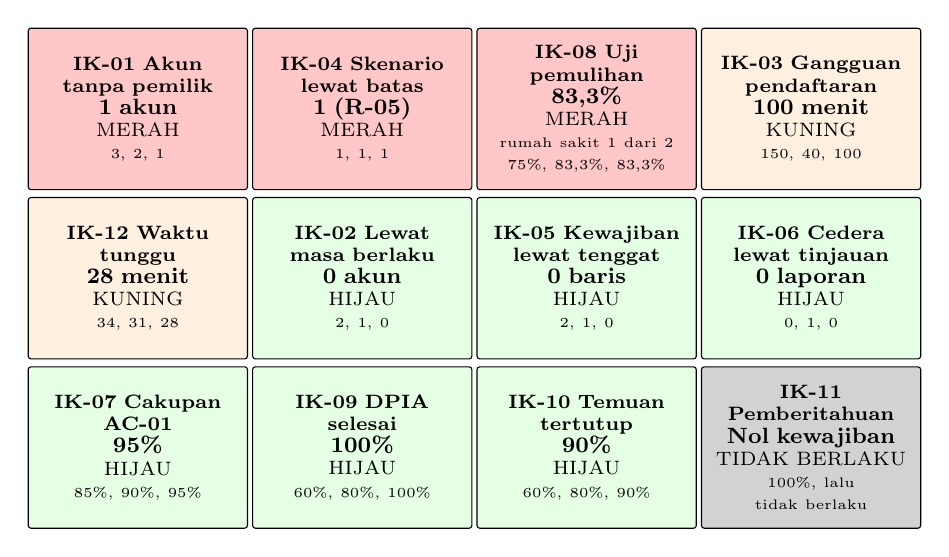
\begin{tikzpicture}[petak/.style={draw, rounded corners=1pt, align=center, text width=2.55cm, minimum height=2.05cm, font=\scriptsize, execute at begin node={\hyphenpenalty=10000}}]
  % Baris disusun dari pengecualian: merah lebih dahulu, lalu kuning, hijau, dan tidak berlaku.
  \node[petak,fill=red!22] at (0,0) {\textbf{IK-01 Akun tanpa pemilik}\\{\footnotesize\textbf{1 akun}}\\MERAH\\{\tiny\mdseries 3, 2, 1}};
  \node[petak,fill=red!22] at (2.85,0) {\textbf{IK-04 Skenario lewat batas}\\{\footnotesize\textbf{1 (R-05)}}\\MERAH\\{\tiny\mdseries 1, 1, 1}};
  \node[petak,fill=red!22] at (5.7,0) {\textbf{IK-08 Uji pemulihan}\\{\footnotesize\textbf{83,3\%}}\\MERAH\\{\tiny\mdseries rumah sakit 1 dari 2}\\{\tiny\mdseries 75\%, 83,3\%, 83,3\%}};
  \node[petak,fill=orange!12] at (8.55,0) {\textbf{IK-03 Gangguan pendaftaran}\\{\footnotesize\textbf{100 menit}}\\KUNING\\{\tiny\mdseries 150, 40, 100}};
  \node[petak,fill=orange!12] at (0,-2.15) {\textbf{IK-12 Waktu tunggu}\\{\footnotesize\textbf{28 menit}}\\KUNING\\{\tiny\mdseries 34, 31, 28}};
  \node[petak,fill=green!10] at (2.85,-2.15) {\textbf{IK-02 Lewat masa berlaku}\\{\footnotesize\textbf{0 akun}}\\HIJAU\\{\tiny\mdseries 2, 1, 0}};
  \node[petak,fill=green!10] at (5.7,-2.15) {\textbf{IK-05 Kewajiban lewat tenggat}\\{\footnotesize\textbf{0 baris}}\\HIJAU\\{\tiny\mdseries 2, 1, 0}};
  \node[petak,fill=green!10] at (8.55,-2.15) {\textbf{IK-06 Cedera lewat tinjauan}\\{\footnotesize\textbf{0 laporan}}\\HIJAU\\{\tiny\mdseries 0, 1, 0}};
  \node[petak,fill=green!10] at (0,-4.3) {\textbf{IK-07 Cakupan AC-01}\\{\footnotesize\textbf{95\%}}\\HIJAU\\{\tiny\mdseries 85\%, 90\%, 95\%}};
  \node[petak,fill=green!10] at (2.85,-4.3) {\textbf{IK-09 DPIA selesai}\\{\footnotesize\textbf{100\%}}\\HIJAU\\{\tiny\mdseries 60\%, 80\%, 100\%}};
  \node[petak,fill=green!10] at (5.7,-4.3) {\textbf{IK-10 Temuan tertutup}\\{\footnotesize\textbf{90\%}}\\HIJAU\\{\tiny\mdseries 60\%, 80\%, 90\%}};
  \node[petak,fill=gray!35] at (8.55,-4.3) {\textbf{IK-11 Pemberitahuan}\\{\footnotesize\textbf{Nol kewajiban}}\\TIDAK BERLAKU\\{\tiny\mdseries 100\%, lalu tidak berlaku}};
\end{tikzpicture}

  \caption{\textit{Dashboard} GRC Medikara, Oktober 2026 (misalkan)}
  \label{fig:ch13-dashboard}
\end{figure}

\begin{table}[!htb]
  \centering\small
  \caption{Tren dua belas indikator, Agustus sampai Oktober 2026 (misalkan)}\label{tab:ch13-tren}
  \begin{tabularx}{\textwidth}{|>{\raggedright\arraybackslash}X|>{\raggedright\arraybackslash}p{0.22\textwidth}|>{\raggedright\arraybackslash}p{0.22\textwidth}|>{\raggedright\arraybackslash}p{0.22\textwidth}|}
    \hline
    \textbf{Indikator} & \textbf{Agustus} & \textbf{September} & \textbf{Oktober} \\ \hline
    IK-01 Akun tanpa pemilik & 3, merah & 2, merah & 1, merah \\ \hline
    IK-02 Lewat masa berlaku & 2, merah & 1, merah & 0, hijau \\ \hline
    IK-03 Gangguan pendaftaran & 150 menit, merah & 40 menit, hijau & 100 menit, kuning \\ \hline
    IK-04 Skenario lewat batas & 1, merah & 1, merah & 1, merah \\ \hline
    IK-05 Kewajiban lewat tenggat & 2, merah & 1, merah & 0, hijau \\ \hline
    IK-06 Cedera lewat tinjauan & 0, hijau & 1, merah & 0, hijau \\ \hline
    IK-07 Cakupan AC-01 & 102/120 = 85\%, merah & 108/120 = 90\%, kuning & 114/120 = 95\%, hijau
    \\ \hline
    IK-08 Uji pemulihan & 9/12 = 75\%; rumah sakit 1/2, merah & 10/12 = 83,33\%; rumah sakit 1/1,
    kuning & 10/12 = 83,33\%; rumah sakit 1/2, merah \\ \hline
    IK-09 DPIA selesai & 3/5 = 60\%, merah & 4/5 = 80\%, kuning & 5/5 = 100\%, hijau \\ \hline
    IK-10 Temuan tertutup & 6/10 = 60\%, merah & 8/10 = 80\%, kuning & 9/10 = 90\%, hijau \\ \hline
    IK-11 Pemberitahuan & 1/1 = 100\%, hijau & Tidak berlaku & Tidak berlaku \\ \hline
    IK-12 Waktu tunggu & 34 menit, merah & 31 menit, merah & 28 menit, kuning \\ \hline
  \end{tabularx}
\end{table}

IK-08 memakai status terburuk dari dua rasio, dengan ambang yang sama: 100 persen hijau, 75 sampai
kurang dari 100 persen kuning, dan kurang dari 75 persen merah. Pada Oktober, 83,33 persen berstatus
kuning, tetapi rumah sakit 1 dari 2 atau 50 persen berstatus merah. Pembacaan ini mengikuti
peringatan Bab 10: gabungan menyamarkan layanan dengan batas gangguan terpendek. Dua belas uji per
bulan membentuk 36 uji triwulan, dengan 29 lulus, sama dengan Bab 10.

Pertanyaan kemudian muncul: bolehkah semua warna dirangkum menjadi satu skor? Dua contoh
menjawabnya:
\begin{enumerate}
  \item Misalkan hijau bernilai 100, kuning 50, merah 0, dan tidak berlaku dikeluarkan. Skor
  gabungannya 16,7 pada Agustus, 27,3 pada September, dan $700 \div 11 \approx 63{,}6$ pada Oktober.
  Skor naik hampir empat kali lipat, sementara IK-01 dan IK-04 merah pada ketiga bulan. Oktober
  bahkan memuat kegagalan uji rumah sakit.
  \item Cakupan AC-01 hijau dan akun tanpa pemilik merah tidak dirata-ratakan menjadi kuning.
  Rata-rata itu tidak berarti apa-apa bagi pemilik Medikara+, karena tidak menunjukkan akun mana
  yang dibekukan.
\end{enumerate}

Bab 5 sudah membahas keterbatasan kategori pada matriks risiko, termasuk resolusi yang buruk
\cite{c05-cox2008}. Skor gabungan warna mewarisi masalah yang sama. Keputusan menolak skor gabungan
punya konsekuensi: laporan bertambah satu baris untuk tiap pengecualian, dan pimpinan tidak mendapat
satu angka yang mudah diingat. Harga itu diterima, karena pesan yang hilang justru pesan yang
dibutuhkan.

\section{Laporan Satu Halaman ke Direksi}

\subsection*{Struktur laporan}

Laporan menghubungkan tiga pesan utama dengan satu keputusan. NIST mengingatkan bahwa ukuran yang
dilaporkan tanpa konteks dapat menimbulkan akibat yang tidak diinginkan atau keraguan. Laporan
karena itu dapat memuat risiko yang ditunjukkan ukuran, kesesuaiannya dengan \textit{risk appetite},
tindakan atau keputusan yang diperlukan, masalah kepatuhan, dan dampaknya pada kesiapan audit
\cite{c13-nist80055v1}. COSO menambahkan bahwa frekuensi mengikuti pembacanya. Pengelola operasi
cocok dengan laporan seketika, manajemen senior dengan laporan yang lebih jarang, dan direksi dengan
laporan yang lebih agregat \cite{c13-coso-kri}. Pada Medikara, \textit{dashboard} dibahas bulanan
pada komite pengarah TI, dan laporan satu halaman terbit triwulanan sesuai 4 laporan pada Bab 2.

Analogi ringkasan rapat membedakan informasi dan keputusan. Daftar kejadian menjelaskan masa lalu.
Usulan dengan pemilik, anggaran, tenggat, dan risiko sisa memberi dasar bertindak.

Dua contoh tentang isi laporan:
\begin{enumerate}
  \item Misalkan laporan menyebut 7 kegiatan selesai. Direksi belum mengetahui dampak, pengecualian,
  dan keputusan yang diperlukan. Membaca 7 baris itu pun tidak mengubah apa pun.
  \item Misalkan laporan meminta direksi menyetujui Rp60 juta untuk rekonsiliasi akun. Permintaan
  itu salah alamat. Bab 2 menempatkan biaya sampai Rp100 juta pada kepala TI, sehingga cukup
  dilaporkan. Waktu direksi dipakai untuk Rp180 juta tahap kedua opsi B, karena keputusan bersyarat
  itu milik direksi pada Bab 10.
\end{enumerate}

Gambar~\ref{fig:ch13-laporan} memperlihatkan susunan satu halaman. Keputusan ditaruh di atas, karena
itu hal pertama yang perlu diketahui pembaca.

\begin{figure}[!htb]
  \centering
  \begin{tikzpicture}[blok/.style={draw, align=left, text width=7.1cm, font=\scriptsize, inner sep=3pt}, catatan/.style={align=left, text width=3.5cm, font=\scriptsize, execute at begin node={\hyphenpenalty=10000}}, panah/.style={-{Stealth[length=2mm]}, thick}]
  \node[blok,fill=praditagreen!15] (kepala) {\textbf{Laporan GRC Triwulan Agustus sampai Oktober 2026}\\{\tiny\mdseries Cakupan, tanggal data, penyusun, dan pemilik laporan}};
  \node[blok,fill=orange!12,below=1.5mm of kepala] (putus) {\textbf{Keputusan yang diminta}\\{\tiny\mdseries Setujui, ubah, atau tolak: tahap kedua Rp180 juta untuk opsi B, paling lambat akhir November 2026}};
  \node[blok,fill=blue!8,below=1.5mm of putus] (p1) {\textbf{Pesan 1: Pemulihan belum memenuhi syarat}\\{\tiny\mdseries 3 dari 5 rumah sakit lulus; R-05 masih 10 persen, batasnya 2 persen}};
  \node[blok,fill=blue!8,below=1mm of p1] (p2) {\textbf{Pesan 2: Akses vendor membaik, belum selesai}\\{\tiny\mdseries Cakupan 95 persen; 1 akun tanpa pemilik dibekukan; TA-01 belum tertutup}};
  \node[blok,fill=blue!8,below=1mm of p2] (p3) {\textbf{Pesan 3: Layanan membaik, masih di bawah target}\\{\tiny\mdseries Waktu tunggu 34, 31, 28 menit; gangguan 150, 40, 100 menit}};
  \node[blok,fill=blue!8,below=1.5mm of p3] (opsi) {\textbf{Tabel tiga pilihan}\\{\tiny\mdseries Biaya, akibat pada risiko, pemilik, tenggat, dan ukuran keberhasilan}};
  \node[blok,fill=green!10,below=1.5mm of opsi] (batas) {\textbf{Batas data dan tindak lanjut}\\{\tiny\mdseries Tingkat lulus uji bukan peluang R-05; 5 uji rumah sakit tergolong sedikit}};
  \draw (kepala.north west) rectangle (batas.south east);
  \node[catatan,right=4mm of putus] (c1) {Dibaca pertama: direksi tahu apa yang harus diputuskan};
  \node[catatan,right=4mm of p2] (c2) {Tiga pesan: angka, tren, dan risiko; tanpa daftar kegiatan};
  \node[catatan,right=4mm of opsi] (c3) {Ada pembanding, sehingga usulan dapat ditolak};
  \node[catatan,right=4mm of batas] (c4) {Batas klaim mencegah tafsir berlebihan};
  \draw[panah] (c1.west) -- (putus.east);
  \draw[panah] (c2.west) -- (p2.east);
  \draw[panah] (c3.west) -- (opsi.east);
  \draw[panah] (c4.west) -- (batas.east);
\end{tikzpicture}

  \caption{Susunan laporan GRC satu halaman (misalkan)}
  \label{fig:ch13-laporan}
\end{figure}

\subsection*{Laporan Medikara: triwulan Agustus sampai Oktober 2026}

Hubungan antarangka berjalan seperti ini. IK-08 memperlihatkan 3 dari 5 rumah sakit lulus. Dua
kegagalan data berasal dari 9 uji akun terpisah. Kedua syarat Bab 10 belum terpenuhi. Peluang R-05
tetap dicatat 0,1, sehingga IK-04 merah. Tingkat lulus uji bukan peluang R-05, sehingga angka 80,6
persen tidak dibaca sebagai peluang apa pun. Tabel~\ref{tab:ch13-keputusan} menyusun pilihannya.

\begin{table}[!htb]
  \centering\small
  \caption{Tiga pilihan untuk tahap kedua opsi B (misalkan)}\label{tab:ch13-keputusan}
  \begin{tabularx}{\textwidth}{|>{\raggedright\arraybackslash}p{0.26\textwidth}|>{\raggedright\arraybackslash}p{0.13\textwidth}|>{\raggedright\arraybackslash}X|>{\raggedright\arraybackslash}X|}
    \hline
    \textbf{Pilihan} & \textbf{Biaya} & \textbf{Akibat pada R-05} & \textbf{Risiko pilihan} \\
    \hline
    1. Tahan tahap kedua; uji ulang 2 rumah sakit dan 9 uji akun terpisah & Rp0 tambahan saat ini &
    Peluang tetap 0,1; harapan kerugian sekitar Rp40 juta lebih tinggi per triwulan & Direksi
    menerima tertulis paparan di atas batas selama satu triwulan \\ \hline
    2. Cairkan Rp180 juta sekarang & Rp180 juta & Peluang tetap dicatat 0,1 sampai uji lulus &
    Syarat direksi hilang; uang keluar sebelum bukti \\ \hline
    3. Hentikan opsi B, kembali ke opsi A & Hemat Rp180 juta & SIMRS pulih 480 menit; batas 2 persen
    dilanggar & Sudah ditolak pada Bab 10 \\ \hline
  \end{tabularx}
\end{table}

\begin{kasus}[title={Kasus Medikara Health: Laporan yang Meminta Satu Keputusan}]
Misalkan kepala risiko menyusun laporan triwulan pada November 2026.

\textbf{Pesan 1.} Pemulihan belum memenuhi syarat. Sebanyak 29 dari 36 uji lulus, tetapi hanya 3
dari 5 rumah sakit. Dua kegagalan data berasal dari 9 uji akun terpisah. R-05 masih 10 persen,
batasnya 2 persen.

\textbf{Pesan 2.} Akses vendor membaik, tetapi belum selesai. Cakupan AC-01 naik 85, 90, 95 persen.
Satu akun tanpa pemilik sudah dibekukan. TA-01 selesai menurut manajemen, dan belum lolos uji ulang.
Tidak ada keputusan yang diminta, karena biayanya berada dalam wewenang kepala TI.

\textbf{Pesan 3.} Layanan membaik, dan masih di bawah target. Waktu tunggu 34, 31, 28 menit, dengan
target 25 menit. Gangguan pendaftaran Oktober 100 menit, di dalam batas 120 menit, tetapi di atas
RTO 90 menit.

\textbf{Keputusan yang diminta.} Setujui pilihan 1 paling lambat akhir November 2026. Pemilik
tindakan kepala operasi TI. Ukuran keberhasilan: 5 dari 5 rumah sakit lulus uji SIMRS di bawah 120
menit, dan 9 dari 9 uji akun terpisah berhasil, paling lambat akhir Januari 2027.

Selisih harapan kerugian R-05 antara 0,1 dan 0,02 adalah Rp160 juta per tahun, atau sekitar Rp40
juta per triwulan. Angka itu harga menunggu bukti. Direksi dapat menolaknya, asalkan penolakan
beserta risiko sisanya dicatat. Bab 14 memasukkan opsi B Rp480 juta ke peta jalan.
\end{kasus}

Laporan yang lebih pendek juga mengubah beban kerja. Tabel~\ref{tab:ch13-beban} menghitungnya pada
tarif Rp60.000 per jam dari Bab 7. Misalkan laporan lama melibatkan 8 unit dengan 6 jam per bulan,
ditambah penyunting 16 jam. Rancangan baru memerlukan 2 jam per indikator per bulan dan 24 jam per
laporan triwulan.

\begin{table}[!htb]
  \centering\small
  \caption{Beban laporan lama dan rancangan baru (misalkan)}\label{tab:ch13-beban}
  \begin{tabularx}{\textwidth}{|>{\raggedright\arraybackslash}X|>{\raggedright\arraybackslash}p{0.27\textwidth}|>{\raggedright\arraybackslash}p{0.27\textwidth}|}
    \hline
    \textbf{Unsur} & \textbf{Laporan 40 halaman} & \textbf{Satu halaman} \\ \hline
    Penyusunan per tahun & $(8 \times 6 + 16) \times 12 = 768$ jam & $12 \times 2 \times 12 + 4
    \times 24 = 384$ jam \\ \hline
    Biaya per tahun & Rp46,08 juta & Rp23,04 juta \\ \hline
    Waktu baca per pembaca & 80 menit, 12 kali & Sekitar 5 menit, 4 kali \\ \hline
  \end{tabularx}
\end{table}

Keputusan mengganti laporan punya dua konsekuensi. Pertama, penghematan 384 jam atau Rp23,04 juta
per tahun berarti indikator ini tidak menambah beban 3.046 jam yang harus dimuat Bab 14. Kedua,
sebagian pembaca kehilangan rincian yang biasa diterima. Rincian itu tetap tersedia di
\textit{dashboard} dan katalog, dan dibaca oleh pihak yang memang bertugas memakainya.

\section{Aktivitas: Dashboard KPI dan KRI serta Laporan Satu Halaman}

\textbf{Tujuan.} Tim menyediakan laporan yang memicu tindakan: katalog 8 sampai 12 indikator,
\textit{dashboard} sederhana, dan laporan satu halaman untuk direksi Medikara atau organisasi tim.

\textbf{Pembagian peran.} Analis risiko memimpin penetapan ambang dan memastikan KRI memakai batas
Bab 5. Anggota berlatar bisnis menyusun narasi untuk direksi. Analis teknologi memeriksa
ketersediaan dan mutu data. Pemilik konteks memastikan penerima laporan memiliki kewenangan atas
keputusan yang diminta.

\textbf{Langkah kerja.}
\begin{enumerate}
  \item Pilih 8 sampai 12 indikator yang mencakup tata kelola, risiko, keamanan, privasi, dan
  kelangsungan layanan. Tulis keputusan yang didukung tiap ukuran. Ukuran tanpa keputusan
  dikeluarkan.
  \item Isi katalog mengikuti kolom \berkas{sources/chapter13/katalog-indikator.csv}. Tetapkan
  rumus, sumber, frekuensi, pemilik, serta ambang tiga warna yang tidak tumpang tindih.
  \item Hitung tiga periode dari \berkas{sources/chapter13/data-indikator.csv}, atau dari data
  organisasi yang sudah dianonimkan. Bedakan nol yang sah, tidak berlaku, dan data tidak tersedia.
  \item Bandingkan hasil dengan \berkas{sources/chapter13/dashboard-contoh.csv}, lalu susun
  \textit{dashboard} pada spreadsheet. Cantumkan angka, kata status, tren, dan perubahan definisi.
  \item Tulis tiga pesan dan satu keputusan melalui
  \berkas{sources/chapter13/templat-laporan-direksi.md}. Nyatakan pilihan, biaya, pemilik, tenggat,
  dan risiko bila ditunda.
  \item Tinjau silang rumus antaranggota, lalu simulasikan rapat 5 menit. Catat apakah direksi
  fiktif dapat memilih tindakan tanpa bertanya apa yang diminta.
\end{enumerate}

\textbf{Luaran.} Katalog indikator, \textit{dashboard}, dan laporan satu halaman.

\textbf{Kaitan dengan capstone.} Luaran masuk tonggak C4 Peta Jalan dan Tata Kelola. Bab 14 memakai
indikator ini sebagai ukuran keberhasilan peta jalan. Metrik layanan diselaraskan dengan IT40713,
dan nilai platform diselaraskan dengan IT40613.

\textbf{Kriteria penilaian.} Kaitan risiko dan keputusan 30 persen; ketepatan definisi dan hitungan
30 persen; ambang dan eskalasi 20 persen; kejelasan permintaan keputusan 20 persen. Hasil tiap tim
boleh berbeda dari contoh. Penilaian berfokus pada penalaran.

\textbf{Berkas pendukung.} Daftar lengkap ada di \berkas{sources/chapter13/README.md}. Data
organisasi nyata wajib seizin organisasi dan dianonimkan. Data pribadi pasien atau karyawan tidak
boleh dipakai.

\begin{pendalaman}
Skrip \texttt{hitung\_indikator.py} menghitung 12 indikator dari data sintetis secara lokal.
Listing~\ref{lst:ch13-status} memperlihatkan aturan penyebut nol dan pembulatan. Nilai penuh
dibandingkan dengan ambang, lalu baru dibulatkan untuk tampilan.

\begin{lstlisting}[basicstyle=\ttfamily\scriptsize,columns=fullflexible,frame=lines,breaklines=true,
  caption={Status rasio, tersedia di \berkas{sources/chapter13/hitung_indikator.py}},
  label={lst:ch13-status}]
def status_rasio(pembilang, penyebut, batas_hijau, batas_kuning):
  """Bandingkan nilai penuh sebelum pembulatan agar ambang tidak bergeser."""
  if pembilang is None or penyebut is None:
    return None, DATA_TIDAK_TERSEDIA
  if pembilang > penyebut:
    raise ValueError("Pembilang melebihi penyebut")
  if penyebut == 0:
    return None, TIDAK_BERLAKU
  nilai = pembilang / penyebut * 100
  if nilai >= batas_hijau:
    return nilai, HIJAU
  if nilai >= batas_kuning:
    return nilai, KUNING
  return nilai, MERAH
\end{lstlisting}

Tim dapat mengotomasi pengambilan dua indikator dari sumber data nyata, misalnya sistem tiket atau
\textit{log}, ke alat \textit{dashboard} sumber terbuka seperti Metabase atau Grafana. Otomasi
memerlukan definisi dan pemeriksaan mutu yang sama. Pengambilan data hanya untuk sistem sendiri atau
yang sudah berizin tertulis. Keberhasilan mengambil data belum membuktikan indikator tepat untuk
keputusan.
\end{pendalaman}

\section{Ringkasan}

KPI, KRI, dan KCI menjawab pertanyaan tentang hasil, paparan, dan kontrol. Data yang sama dapat
mendukung beberapa keputusan bila definisi dan batas tafsirnya jelas. Cakupan AC-01 yang naik sampai
95 persen tidak meniadakan 1 akun tanpa pemilik. Indikator yang mendahului memberi waktu untuk
bertindak, sedangkan indikator yang tertinggal mencatat hasil yang tetap perlu dipertanggungjawabkan
secara terbuka.

Indikator yang baik memiliki pembilang, penyebut, cakupan, tanggal, sumber, pemilik, dan tindakan.
Perbedaan 108 dari 108 dengan 108 dari 120 berasal dari penyebut, bukan dari pekerjaan. Data tidak
tersedia dan penyebut nol tidak boleh diperlakukan sebagai kinerja sempurna. Mutu data diperiksa
oleh pihak di luar penghasil angka, karena ukuran dengan target mendorong orang menyesuaikan
catatan.

Ambang diturunkan dari batas Bab 5 dan memberi waktu merespons. Tidak semua indikator memerlukan
tiga warna. Toleransi nol tetap merah sampai nol, sehingga peringatan dini berpindah ke indikator
lain. Pada IK-03, RTO 90 menit dan batas 120 menit membentuk zona kuning yang berasal dari keputusan
terdahulu. Jalur eskalasi mengikuti batas delegasi Bab 2, sehingga indikator tidak menciptakan
wewenang baru.

Portofolio 12 indikator dipilih dari 46 usulan pada contoh Medikara, dan bahan Bab 8 sampai Bab 12
dipilah menurut pembacanya. \textit{Dashboard} menunjukkan keadaan, tren, dan pengecualian pada satu
halaman, tanpa skor gabungan. Skor 63,6 pada Oktober terlihat membaik, padahal dua KRI merah pada
ketiga bulan dan satu KCI gagal pada rumah sakit.

Laporan direksi mengajukan pilihan yang dapat diputuskan. Medikara tidak meminta persetujuan Rp60
juta yang berada dalam wewenang kepala TI, tetapi meminta keputusan atas Rp180 juta tahap kedua opsi
B, dengan harga menunggu sekitar Rp40 juta per triwulan. Pesan utama bab ini: indikator berguna
ketika mengubah keputusan dan tindakan, bukan ketika memenuhi halaman laporan.

\section{Latihan}

\subsection*{Latihan 1: Aktivitas atau Risiko}

``Jumlah pelatihan keamanan yang diselenggarakan'' diusulkan sebagai KRI. Kritisi usulan ini dan
tawarkan indikator yang lebih baik. Latihan ini membuktikan bahwa ukuran kegiatan belum tentu
menggambarkan paparan risiko. NIST memberi arah serupa: pelatihan kesadaran keamanan dinilai dari
tingkat penyelesaian dan hasil kuis, bukan dari label partisipasi rendah, sedang, atau tinggi
\cite{c13-nist80055v1}.
\begin{enumerate}
  \item Tetapkan risiko dan perilaku yang hendak diubah.
  \item Bandingkan jumlah acara dengan cakupan dan hasil uji.
  \item Usulkan rumus, ambang, dan keputusan yang dipicunya.
\end{enumerate}

Tabel~\ref{tab:ch13-lat1-contoh} memberi contoh terisi, dan Tabel~\ref{tab:ch13-lat1-hasil} menjadi
lembar isian.

\begin{table}[!htb]
  \centering\small
  \caption{Contoh terisi Latihan 1 (misalkan)}\label{tab:ch13-lat1-contoh}
  \begin{tabularx}{\textwidth}{|>{\raggedright\arraybackslash}X|>{\raggedright\arraybackslash}p{0.25\textwidth}|>{\raggedright\arraybackslash}X|}
    \hline
    \textbf{Ukuran} & \textbf{Nilai contoh} & \textbf{Batas tafsir} \\ \hline
    Pelatihan diselenggarakan & 12 acara & Tidak menunjukkan siapa belajar \\ \hline
    Cakupan pegawai prioritas & $30 / 100 = 30$ persen & Hadir belum berarti paham \\ \hline
    Peserta lulus uji & $24 / 30 = 80$ persen & Hanya berlaku bagi peserta \\ \hline
    Usulan KRI: pegawai prioritas belum lulus dalam 12 bulan & $100 - 24 = 76$ pegawai & Memicu
    penjadwalan; belum membuktikan perilaku \\ \hline
  \end{tabularx}
\end{table}

\begin{table}[!htb]
  \centering\small
  \caption{Lembar isian Latihan 1}\label{tab:ch13-lat1-hasil}
  \begin{tabularx}{\textwidth}{|>{\raggedright\arraybackslash}X|>{\raggedright\arraybackslash}p{0.25\textwidth}|>{\raggedright\arraybackslash}X|}
    \hline
    \textbf{Ukuran} & \textbf{Nilai} & \textbf{Batas tafsir} \\ \hline
    \dots & \dots & \dots \\ \hline
    \dots & \dots & \dots \\ \hline
    \dots & \dots & \dots \\ \hline
  \end{tabularx}
\end{table}

Hasil dapat berbeda. Penilaian bertumpu pada alasan dan perbandingan bukti.
\begin{enumerate}
  \item Pada contoh, mengapa 80 persen lulus uji tidak berarti 80 persen pegawai prioritas
  terlindungi?
  \item Data apa yang diperlukan sebelum menyimpulkan risiko turun?
  \item Bagaimana mencegah target mendorong manipulasi jumlah peserta?
\end{enumerate}

\subsection*{Latihan 2: Menurunkan Ambang Akses}

Turunkan ambang KRI untuk risiko kontrol akses dari pernyataan \textit{risk appetite} yang dibuat
pada Pertemuan 5. Latihan ini membuktikan bahwa toleransi, ambang, dan eskalasi harus konsisten.
\begin{enumerate}
  \item Salin pernyataan toleransi dan cakupannya dari luaran Pertemuan 5.
  \item Tentukan nilai yang melewati toleransi, pemilik, dan tindakan.
  \item Tetapkan indikator pendamping yang memberi peringatan dini.
  \item Uji ambang pada tiga periode.
\end{enumerate}

Tabel~\ref{tab:ch13-lat2-contoh} memberi contoh terisi dari batas nol akun pada Bab 5, dan
Tabel~\ref{tab:ch13-lat2-hasil} menjadi lembar isian.

\begin{table}[!htb]
  \centering\small
  \caption{Contoh terisi Latihan 2 (misalkan)}\label{tab:ch13-lat2-contoh}
  \begin{tabularx}{\textwidth}{|>{\raggedright\arraybackslash}p{0.14\textwidth}|>{\raggedright\arraybackslash}p{0.12\textwidth}|>{\raggedright\arraybackslash}p{0.16\textwidth}|>{\raggedright\arraybackslash}p{0.13\textwidth}|>{\raggedright\arraybackslash}X|}
    \hline
    \textbf{Periode} & \textbf{IK-01} & \textbf{IK-02} & \textbf{IK-07} & \textbf{Status dan
    tindakan} \\ \hline
    Agustus & 3 akun & 2 akun & 85 persen & Semua merah; bekukan akun, periksa daftar \\ \hline
    September & 2 akun & 1 akun & 90 persen & IK-07 kuning; IK-01 dan IK-02 tetap merah \\ \hline
    Oktober & 1 akun & 0 akun & 95 persen & IK-07 dan IK-02 hijau; IK-01 tetap merah \\ \hline
  \end{tabularx}
\end{table}

\begin{table}[!htb]
  \centering\small
  \caption{Lembar isian Latihan 2}\label{tab:ch13-lat2-hasil}
  \begin{tabularx}{\textwidth}{|>{\raggedright\arraybackslash}p{0.14\textwidth}|>{\raggedright\arraybackslash}p{0.12\textwidth}|>{\raggedright\arraybackslash}p{0.16\textwidth}|>{\raggedright\arraybackslash}p{0.13\textwidth}|>{\raggedright\arraybackslash}X|}
    \hline
    \textbf{Periode} & \textbf{KRI} & \textbf{Pendamping} & \textbf{KCI} & \textbf{Status dan
    tindakan} \\ \hline
    \dots & \dots & \dots & \dots & \dots \\ \hline
    \dots & \dots & \dots & \dots & \dots \\ \hline
    \dots & \dots & \dots & \dots & \dots \\ \hline
  \end{tabularx}
\end{table}

Hasil dapat berbeda. Penilaian bertumpu pada alasan dan perbandingan bukti.
\begin{enumerate}
  \item Mengapa tren 3, 2, 1 belum berarti risiko diterima?
  \item Apa status bila nol akun terlapor tetapi ekstrak satu rumah sakit tidak lengkap?
  \item Pada Oktober, IK-02 hijau dan IK-01 merah. Apa yang dibaca pemilik Medikara+ dari pasangan
  itu?
\end{enumerate}

\subsection*{Latihan 3: Laporan yang Memicu Keputusan}

Jelaskan apa yang membuat sebuah laporan direksi berujung pada keputusan, bukan sekadar dibaca.
Latihan ini membuktikan bahwa opsi dan konsekuensi yang jelas lebih berguna dari daftar kegiatan.
\begin{enumerate}
  \item Pilih satu pengecualian penting dari \textit{dashboard}.
  \item Periksa batas delegasi Bab 2, lalu pastikan keputusannya memang milik penerima laporan.
  \item Tulis rekomendasi dan pembanding, lengkap dengan biaya dan risiko.
  \item Nyatakan pemilik, tenggat, dan ukuran keberhasilan.
\end{enumerate}

Tabel~\ref{tab:ch13-lat3-contoh} memberi contoh terisi, dan Tabel~\ref{tab:ch13-lat3-hasil} menjadi
lembar isian.

\begin{table}[!htb]
  \centering\small
  \caption{Contoh terisi Latihan 3 (misalkan)}\label{tab:ch13-lat3-contoh}
  \begin{tabularx}{\textwidth}{|>{\raggedright\arraybackslash}p{0.19\textwidth}|>{\raggedright\arraybackslash}X|>{\raggedright\arraybackslash}X|}
    \hline
    \textbf{Unsur} & \textbf{Usulan contoh} & \textbf{Bukti} \\ \hline
    Keputusan & Tahan tahap kedua opsi B, uji ulang satu triwulan & 3 dari 5 rumah sakit lulus; 2
    data gagal dari 9 uji \\ \hline
    Pembanding & Cairkan Rp180 juta sekarang & Peluang R-05 tetap dicatat 0,1 sampai uji lulus \\
    \hline
    Harga menunggu & Sekitar Rp40 juta per triwulan & (Rp200 juta dikurangi Rp40 juta) dibagi 4 \\
    \hline
    Keberhasilan & 5 dari 5 rumah sakit; 9 dari 9 uji akun terpisah & Hasil uji yang disahkan
    pemilik layanan \\ \hline
  \end{tabularx}
\end{table}

\begin{table}[!htb]
  \centering\small
  \caption{Lembar isian Latihan 3}\label{tab:ch13-lat3-hasil}
  \begin{tabularx}{\textwidth}{|>{\raggedright\arraybackslash}p{0.19\textwidth}|>{\raggedright\arraybackslash}X|>{\raggedright\arraybackslash}X|}
    \hline
    \textbf{Unsur} & \textbf{Usulan} & \textbf{Bukti} \\ \hline
    \dots & \dots & \dots \\ \hline
    \dots & \dots & \dots \\ \hline
    \dots & \dots & \dots \\ \hline
  \end{tabularx}
\end{table}

Hasil dapat berbeda. Penilaian bertumpu pada alasan dan perbandingan bukti.
\begin{enumerate}
  \item Apa yang hilang dari laporan bila baris biaya dihapus?
  \item Bagaimana mencatat penolakan direksi beserta risiko sisanya?
  \item Pada contoh, apa yang berubah bila uji ulang hanya meluluskan 4 dari 5 rumah sakit?
\end{enumerate}
